% *********************************************************************
% © 2026 Jeremy Sylvestre
%
% Permission is granted to copy, distribute and/or modify this document
% under the terms of the GNU Free Documentation License, Version 1.3 or
% any later version published by the Free Software Foundation; with no
% Invariant Sections, no Front-Cover Texts, and no Back-Cover Texts. A
% copy of the license is included in the appendix entitled “GNU Free
% Documentation License” that appears in the output document of this
% PreTeXt source code. All trademarks™ are the registered® marks of
% their respective owners.
%
% *********************************************************************
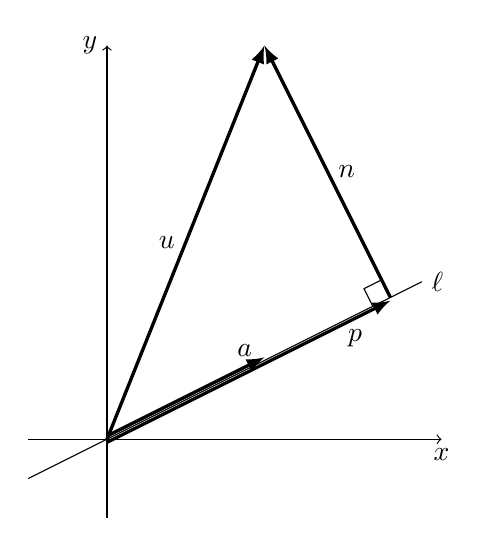
\begin{tikzpicture}[
	vector/.style={-latex,very thick},
	% scale=0.75
]
	\coordinate (o) at (0,0);
	\coordinate (u) at (2,5);
	\coordinate (a) at (2,1);
	\coordinate (p) at (3.6,1.8);

	\draw[->] (-1,0) to (4.25,0) node[below] {$x$};
	\draw[->] (0,-1) to (0,5) node[left] {$y$};

	% parallel to (2,1)
	\draw[thin] (-1,-0.5) to (4,2) node[right] {$\ell$};

	\draw[vector] (o) to node[left] {$\uvec{u}$} (u);
	\draw[vector] ([yshift=0.04cm]o) to node[above,very near end] {$\uvec{a}$} ([yshift=0.04cm]a);
	\draw[vector] ([yshift=-0.04cm]o) to node[below,very near end] {$\uvec{p}$} ([yshift=-0.04cm]p);
	\draw[vector] (p) to node[right] {$\uvec{n}$} (u);

	% perp symbol
	\begin{scope}[xshift=3.6cm,yshift=1.8cm]
		\draw[thin,rotate=26.565] (-0.25,0) to (-0.25,0.25) to (0,0.25);
	\end{scope}

\end{tikzpicture}
